\documentclass{article}


% if you need to pass options to natbib, use, e.g.:
    \PassOptionsToPackage{numbers, compress}{natbib}
% before loading neurips_2023


% ready for submission
% \usepackage{neurips_2023}


% to compile a preprint version, e.g., for submission to arXiv, add add the
% [preprint] option:
    \usepackage[preprint]{neurips_2023}


% to compile a camera-ready version, add the [final] option, e.g.:
    % \usepackage[final]{neurips_2023}


% to avoid loading the natbib package, add option nonatbib:
%    \usepackage[nonatbib]{neurips_2023}


\usepackage[utf8]{inputenc} % allow utf-8 input
\usepackage[T1]{fontenc}    % use 8-bit T1 fonts
\usepackage{hyperref}       % hyperlinks
\usepackage{url}            % simple URL typesetting
\usepackage{booktabs}       % professional-quality tables
\usepackage{amsfonts}       % blackboard math symbols
\usepackage{nicefrac}       % compact symbols for 1/2, etc.
\usepackage{microtype}      % microtypography
\usepackage{xcolor}         % colors
\usepackage{amsmath}
\usepackage{amssymb}
\usepackage{graphicx}
\usepackage{makecell}

\usepackage{algorithm}
\usepackage{algorithmic}
\usepackage{utfsym}
\newcommand{\xmark}{\usym{2717}}



\title{Meta-learning Implicit Neural Representation for Sparse Time Series Functional Data Analysis}


% The \author macro works with any number of authors. There are two commands
% used to separate the names and addresses of multiple authors: \And and \AND.
%
% Using \And between authors leaves it to LaTeX to determine where to break the
% lines. Using \AND forces a line break at that point. So, if LaTeX puts 3 of 4
% authors names on the first line, and the last on the second line, try using
% \AND instead of \And before the third author name.


% \author{%
%   David S.~Hippocampus\thanks{Use footnote for providing further information
%     about author (webpage, alternative address)---\emph{not} for acknowledging
%     funding agencies.} \\
%   Department of Computer Science\\
%   Cranberry-Lemon University\\
%   Pittsburgh, PA 15213 \\
%   \texttt{hippo@cs.cranberry-lemon.edu} \\
  % examples of more authors
  % \And
  % Coauthor \\
  % Affiliation \\
  % Address \\
  % \texttt{email} \\
  % \AND
  % Coauthor \\
  % Affiliation \\
  % Address \\
  % \texttt{email} \\
  % \And
  % Coauthor \\
  % Affiliation \\
  % Address \\
  % \texttt{email} \\
  % \And
  % Coauthor \\
  % Affiliation \\
  % Address \\
  % \texttt{email} \\
% }

\author{%
  Bofan Chen\\
  Department of Pure Mathematics and Mathematical Statistics\\
  University of Cambridge\\
  \texttt{cbfcbf.byron@gmail.com} \\}
\begin{document}


\maketitle

\begin{abstract}
  Sparse time series data is everywhere in our daily life, which is formed by sparsely observed samples from a given function distribution. However, traditional statistical methods struggle to analyze such data effectively. 
  Here, we introduce MetaINR, a method for learning the implicit neural representation (INR) of time series from sparse and irregular observations.
  MetaINR incorporates meta-learning into the functional data analysis (FDA) framework, 
  efficiently learning sample distributions. 
  It utilizes a specific SIREN-based network architecture to recover complete samples based on a few observation points. 
  With MetaINR, estimations of the mean function, covariance operator, and principal components become straightforward.
  Our experiments, conducted on both synthetic and real data, demonstrate that MetaINR significantly outperforms traditional baseline methods in terms of estimation accuracy.
\end{abstract}

\section{Introduction}
Sparse time series data is common in daily life, such as medical data measured at different times for patients or height data collected at various stages of adolescence. 
However, the sparsity and irregularity of such data make traditional statistical methods hard to apply directly. 
Additionally, the consideration of continuity and differentiability properties in most time series data pose challenges for multivariable statistical analysis.

Recent research suggests that meta-learning \cite{finn2017model,hospedales2021meta,beck2023survey} exhibits great advantages in handling sparse data. 
It possesses the capability to identify shared patterns among related tasks \cite{raghu2019rapid}, 
facilitating few-shot learning or even one-shot learning \cite{sun2019meta} with extremely limited training data. 
Moreover, there has been substantial progress in statistical analysis utilizing dense functional data to address continuous time series issues \cite{wang2016functional}. 
\textcolor{blue}{These findings inspire us to leverage meta-learning techniques to transform sparse time series samples into dense formats (recover the samples).
Subsequently, we can extend the established functional data analysis methodologies tailored for dense data to analyze sparse time series datasets effectively.
}

In this paper, we introduce a novel approach, MetaINR, which combines meta-learning and functional data analysis to address the estimation challenges posed by sparse time series data. 
Through this method, we use meta-learning to realize the implicit neural representation (INR) to
reconstruct the time series function for each sample based on sparse time series observations.
Furthermore, we can estimate the mean, covariance, and principal components of the distribution behind these samples.
\textcolor{blue}{
  The advantange of MetaINR can be summarized as follows:
  \begin{itemize}
    \item Efficient and accurate reconstruction of time series samples with sparse observations by leveraging information from the entire dataset
    \item Effective estimation of mean function, covariance operator and principal components for sparse time series dataset
    \item Independence from any initial assumptions about the distribution of time series samples
    \item Preservation of fine details in the samples and easy calculation for their derivatives through the SIREN-based INR
  \end{itemize}
}

Therefore, MetaINR method provides a new solution for analyzing sparse time series data.


% Sparse time series data 在日常生活中非常常见,比如病人在不同时间测量的医疗数据、青少年在成长时不同阶段测量得到的身高数据等。这些数据的稀疏性和irregularity让传统的统计手段变得不太适用。同时,绝大多数时间序列数据所拥有的连续性,可微性等性质也给基于multivarible的统计学分析带来了困境
% 最近的研究表明,元学习在处理稀疏形数据中具有独特的优势。它可以从大量相似的任务中学习任务的共性,并对非常稀疏的训练集做到few-shot learning, 甚至 one-shot learning。同时,在处理连续的时间序列问题时,基于funcitonal data 的统计学也逐渐成熟。
% 在本文中,我们结合了meta-learning和functional data analysis的方法首次提出了metaINR,来解决对稀疏时间序列数据的估计问题。通过这个方法,我们可以基于多个样本的稀疏的时间序列观测较好地重构每个样本的时间序列函数,并且进一步地估算这些样本分布的均值、协方差和主成分。
% metaINR为处理稀疏时间序列问题给出了新的解决方案。
\section{Related works}

\subsection{Functional Data Analysis (FDA)}

% Traditional multivariate statistics 把一个有限维空间中的向量作为研究对象,来分析它的统计性质,如均值向量、协方差矩阵等。在维度较小的时候,这并没有什么不妥。然而如果把分析对象所在空间的维度提高到无穷维,比如L2空间时,传统方法将会面临一些挑战。在函数空间,人们的关注点并不会局限于向量在某个维度上的取值,人们还会关注连续性、导数等更多性质。同时,随着空间增长到无穷维,原先多元统计中的很多指标也会丧失意义,如概率密度函数等。正是由于无穷维和有穷维空间的统计性质和人们关注点的不同,functional data analysis(FDA) 这个方向引起了研究者的广泛关注。
\textbf{Multivariate data versus functional data} 
Traditional multivariate statistics take finite-dimensional vectors as the objects of study to analyze their statistical properties, such as mean vectors and covariance matrices. 
This approach is appropriate and is easy to compute when the dimension of the statistical objects is relatively small. 
However, if the dimension of the space is increased to infinite, for example, in $L^2$ space, traditional methods face certain challenges. 
Besides the expensive computational cost, in such functional spaces, people's focus is not only on the values of vectors in a particular dimension but also on properties such as continuity, smoothness and derivatives. 
Additionally, as the space grows to infinite dimensions, many useful tools in multivariate statistics, such as probability density functions, will lose their meaning. 
It is the differences in statistical properties and people's focus between infinite-dimensional and finite-dimensional spaces, that have led to widespread attention to functional data analysis (FDA) \cite{wang2016functional,kokoszka2017introduction} among researchers.
In FDA, scientists treat functions as basic elements for analysis and have developed various methods to estimate the statistical properties for a functional distribution, such as mean function, covariance operator and functional principal components.

% Time series是一个很典型的需要在无穷维函数空间中处理的研究对象。这是因为现实中收集的时间序列数据往往具有连续性,同时,在某些情况下,人们会关注它的导数、时间对齐(registration)等话题。有很多之前的研究基于多元统计学对时间序列进行分析。比如···。从函数逼近的观点来看,这些基于多元统计的研究确实能够很好的反映一些时间序列的性质,但是这在很多情况下是比较难以推广的,比如本文中所研究的sparse time series data。
\textbf{Sparse time series data}
Time series is a typical object that needs to be addressed in an infinite-dimensional function space. 
This is because time series data collected in reality often exhibit irregularity and continuity, and, in certain situations, people may focus on topics such as derivatives and time alignment (registration).
Many previous time series models were limited to multivariate statistical methods, such as Vector AutoRegression (VAR)\cite{stock2001vector}, AutoRegressive Integrated Moving Average model (ARIMA) \cite{box2015time}, Generalized AutoRegressive Conditional Heteroskedasticity (GARCH) \cite{francq2019garch}, to name a few.
From the perspective of function approximation, these multivariate-statistics-based studies can indeed reflect certain properties of time series. 
However, in many cases, this approach is challenging to generalize, as is the case with sparse time series data.
% 当人们对time series的观测频率不高并且不规律的时候,就会形成sparse time series data。这种类型的数据在医学领域中尤其常见,因为人们只有在医院才会采集数据,而往往看病的次数是因人而异的,看病频率的也是不规律的。如果要用多元统计学分析这种类型的“杂乱”数据,人们往往会束手无策。在functional data analysis中,人们可以通过local polynomial regression的方法先估计出函数形数据的原始形式,然后在这个基础上估计均值,协方差算子等统计量(详见appendix)。local polynomial regression可以表示如下:
When the observation frequency of time series is low and irregular, sparse time series data is formed. 
We can represent the sparse dataset of $n$ samples as 
$$
D=\{(t_{ij},y_{ij})_{j=1}^{J_i}\}_{i=1}^n
$$

where
$y_{ij}=x_i(t_{ij}) , i=1, \cdots, n, j=1, \cdots, J_i$ and $J_i$ is the total observations of the $i$-th sample.
This type of data is particularly common in the medical field \cite{holte2012efficient,muller2005functional}, as the frequency of medical visits varies from person to person, with irregular patterns.
%由于irregularity和sparsity,这种形式的data已经完全不能够用传统的多元统计方法或者是dense-data-based FDA来分析了,而需要引入新的方法。
Due to irregularity and sparsity, this form of data cannot be analyzed using traditional multivariate statistical methods or dense-data-based functional data analysis (FDA). Instead, it requires the introduction of new methods.

\textcolor{blue}{
\textbf{Our benchmarks and the drawbacks of traditional FDA method for sparse data}
There have been previous explorations in sparse functional data analysis. 
We introduce the following two traditional solutions for sparse time series data as benchmarks in this paper:
\begin{itemize}
  \item \textbf{Local polynomial regression + dense-data-based FDA (Pre-smoothing method)}: 
  In this method, we first utilize local polynomial regression directly to recover samples with sparse observations, 
  and then we apply dense-data-based methods to the recovered dense samples. 
  However, this method is inherently unreliable due to the extremely sparse observations for individual samples in the dataset. 
  This sparsity leads to unreliable local polynomial reconstructions, 
  undermining the overall reliability of the method.
  % \textcolor{red}{[TODO bandwidth choose problem]} 
  \item \textbf{Principal Analysis by Conditional Expectation (PACE method) }\cite{yao2005functional}: 
  In this method, we start by employing local polynomial regression to estimate the mean function and variance kernel. 
  Next, we calculate principal components based on these estimates. 
  Finally, we recover samples by computing the scores associated with each principal component (see details in the appendix).
  Comparing to Pre-smoothing method, this approach leverages information from observations of other samples in the dataset during the sample recovery process, 
  thereby enhancing the reliability of the reconstruction. 
  However, it's important to note that PACE also comes with limitations, primarily because it heavily depends on the assumption that scores follow a normal distribution while recovering time series samples.
\end{itemize}
%我们引入以下两种对sparse time series data的传统解决方案作为本文的benchmarks
%1.local polynomial reconstruction + dense-data-based approach: 先直接利用local polynomial regression 对拥有稀疏observaiton的sample进行recover, 然后再利用dense-data-based 的方法对函数形数据进行分析
%显然,这是不可靠的。这是因为数据集中对于单个样本的观测是极为稀疏的,基于稀疏样本的local polynomial reconstruction会变得非常不可靠。
%2.PACE: 先利用local polynomial regression估计均值函数和方差核,然后计算主成分,利用主成分恢复样本。 这种方法在恢复sample时结合数据集中其他样本的信息,因此基于PACE的reconstruction会变得相对可靠。然而,PACE方法也有不足之处,它在恢复时间序列样本的过程中较大程度地依赖了分数服从正态分布的假设。
}

\subsection{Machine learning for functional data}
% 与传统方法不同的是,本文将引入Machine learning的方法来analyze sparse time series data。具体而言,这涉及到两个方面。1. 我们将采用INR来恢复并且表示每一个sample;2. 我们将借助meta-learning的方法利用全数据集的信息对每个sample的INR进行有效的估计。
Unlike traditional methods, this paper introduces machine learning techniques to analyze sparse time series data. 
Specifically, this involves two aspects:
\begin{itemize}
  \item We will use Implicit Neural Representation (INR) \cite{sitzmann2020implicit} to recover and represent each sample.
  \item We will leverage meta-learning methods to effectively estimate the INR for each sample with sparse observations.
\end{itemize}

\subsubsection{Implicit Neural Representation}

% 传统上,函数形数据的表示会用标准的网格法,即给定有限个坐标和函数值的pairs(ti,yi)。这么做有一定的缺陷:原来在无穷维空间中的函数形数据被离散化到了有穷维空间,它不仅不利于求导等计算,而且会极大影响函数的在一个较小时间区间上的分辨率。随着深度学习的兴起,人们发现可以利用深度神经网络来表示函数。···
\textbf{Traditional grid-based representation versus implicit neural representation}
% Our method introduce the implicit neural representation (INR) to represent functional data for further analysis. 
Traditionally, the representation of functional data $y(t)$ involves using a standard grid-based method, 
wherein a finite set of coordinates and corresponding function values are given as pairs $(t_i, y_i)$. 
However, this approach has certain drawbacks: the original functional data in an infinite-dimensional space is discretized into a finite-dimensional space. 
This not only hampers operations like differentiation but also significantly impacts the resolution of the function within a smaller time interval.
With the emergence of deep learning, it has been discovered that utilizing deep neural networks can be an effective way to represent functions implicitly.
Implicit neural representation (INR) parameterize the functional data by deep neural networks:
$$y(t)=F_\phi(t), $$
where $F_\phi(\cdot)$ is a deep neural network parameterized by $\phi$.
This type of continuous representation not only proves to be more memory-efficient but also enables higher resolution and the handling of more complex operations on functional data.

%【】提出了SIREN的函数结构,。
\textbf{SIREN architecture for time series and its advantages}
% 很多之前的工作用Relu-based multilayer perceptrons(MLP) 来作为INR的神经网络架构,但是基于这种架构的INR往往缺乏表达信号中精细细节的能力,并且不能很好的表示目标信号的多阶导数。为了解决这个问题,【1】提出了SIREN的架构来替代传统的ReLU-MLPs。它使用sine函数来作为神经网络的激活函数,可以很好的刻画函数的细节。令人惊奇的是,当对用SIREN来表示函数求导后,它依然可以用SIREN来表示。虽然之前的研究大多利用SIREN来表示图像和视频,却很少用来表示时间序列。本文将SIREN用在时间序列的分析中,我们发现SIREN在表示时间序列上具有优越性。
Many prior works have utilized ReLU-based multilayer perceptrons (MLP) as the neural network architecture for Implicit Neural Representations (INR) \cite{genova2019learning,park2019deepsdf}. 
However, ReLU-based INR often lack the ability to capture fine details in signal and struggle to effectively express higher-order derivatives.
In addressing these limitation, \cite{sitzmann2020implicit} introduced the SIREN architecture as an alternative to traditional ReLU-MLPs:
$$
\Phi(\mathbf{x})=\mathbf{W}_n\left(\phi_{n-1} \circ \phi_{n-2} \circ \ldots \circ \phi_0\right)(\mathbf{x})+\mathbf{b}_n, \quad \mathbf{x}_i \mapsto \phi_i\left(\mathbf{x}_i\right)=\sin \left(\mathbf{W}_i \mathbf{x}_i+\mathbf{b}_i\right)
$$
where $\phi_i: \mathbb{R}^{M_i} \mapsto \mathbb{R}^{N_i}$ is the $i^{t h}$ layer of the network with weight matrix $\mathbf{W}_i \in \mathbb{R}^{N_i \times M_i}$ and biases $\mathbf{b}_i \in \mathbb{R}^{N_i}$.
SIREN employs the sine function as the activation function, effectively modeling signals with fine details.
A remarkable observation is that even after taking derivatives of a function represented using SIREN, 
it can still be expressed using the SIREN architecture. 
These properties of SIREN make it the preferred choice for INR.
While previous research predominantly applied SIREN to represent images and videos \cite{lee2021meta}, its application in time series representation has been limited. 
Inspired by these and other seminal works, this paper explores the use of SIREN-based INR of time series samples and demonstates its superiority in further FDA analysis.


\subsubsection{Meta-learning for sparse data INR}

\textbf{Meta-learning framework}
Meta-learning was initially introduced to enhance the efficiency of machine learning, often referred to as ``learning to learn''.
By employing the deep learning model $F_\phi(\cdot)$ to address similar tasks, the ``shared characteristics'' among these tasks can be leveraged to expedite the machine learning process \cite{raghu2019rapid}.
% Meta-learning 一开始被提出是为了提高机器的学习效率,即learning to learn。 使用同一个模型来解决一系列相似的task,往往可以利用这些相似任务的”共性“来帮助机器更快地完成训练。
To fomulate, given the observation dataset $D^*$ of the target task and the observation dataset $D=\bigcup_{i=1}^n D_i$ of $n$ similar tasks, we need to find a meta-function to effectively learn the parameters of the given task, namely $\phi^*=f_\theta(D^*)$,
where $\theta$ is the meta-parameter of the meta-function $f_\theta(\cdot)$ that can be learned from $D$. Accordingly, the original target task can be solved as $F_{\phi^*}(\cdot)$.
In fact, the representation of meta-function $f_\theta(\cdot)$ can be diverse. There are two main classes of methods \cite{beck2023survey}:  Parameterized Policy Gradient Methods (PPG) and Black Box Methods.

\textbf{Parameterized Policy Gradient Methods and MAML}
The PPG method use an iterative algorithm to represent $f_\theta$, which has an innerloop of the form:
$$
\phi^*_{j+1}=\phi_j^*-\alpha_\theta \nabla_{\phi_j^*} \hat{L}_\theta\left(D^*, F_{\phi_j^*}\right),
$$
with the initial value $\phi_0^*=\phi_0^*(\theta)$.
This is very intuitive because it is similar to the traditional gradient decent method to optimize. 
The only difference is that the initial value, loss function and gradient step should be carefully trained by the observations of other tasks $D$ in this scenario.
One important example of PPG method is  Model-Agnostic Meta-Learning (MAML) \cite{finn2017model}, where $\phi_0^*(\theta)=\theta$ and $\hat{L}_\theta$ can be any loss function independent of $\theta$.
MAML can be regarded as learning an initial value for a task distribution, which retains the gradient decent framework of traditional optimization algorithms.

\begin{figure}[tb]
  \centering
  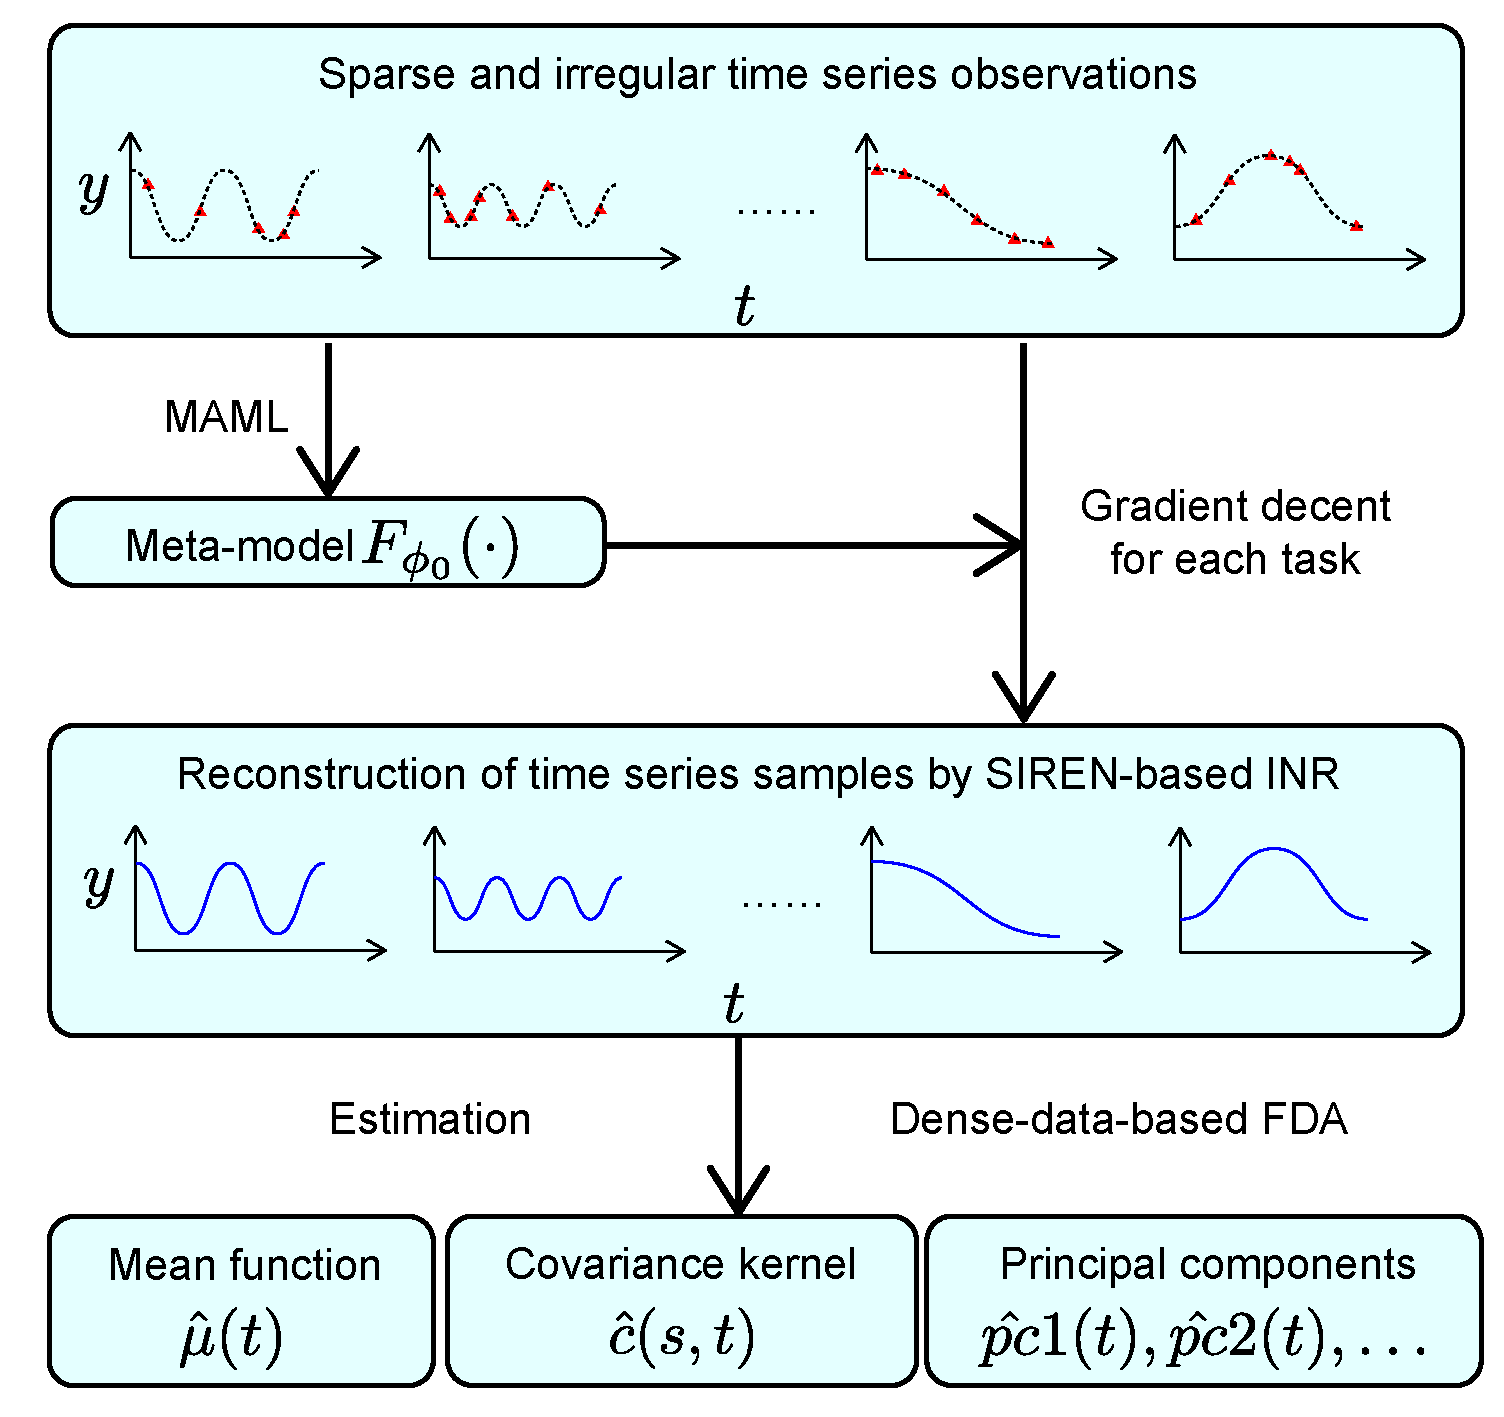
\includegraphics[width=0.8\textwidth]{illustration.pdf}
  \caption{\textbf{MetaINR workflow.} Given the sparse and irregular observations from several samples of an functional distribution, MAML algorithm is implemented to learning the optimal initial value $\phi_0$ for SIREN architecture $F$. The meta-model $F_{\phi_0}$ contain the ``shared characteristics'' from the distribution, hence the recovery of samples can be implemented efficiently and accurately.
  The dense-data-based FDA methods then can be applied effectively on the INRs of samples, such as the estimation of mean function, covariance kernel and principal components.}
  \label{MetaINR workflow}
\end{figure}

\textbf{Black box methods}
Since we only care about the target function $F_\phi(\cdot)$ rather than the value of parameters $\phi$, an alternative way to treat $f_\theta(\cdot)$ is to see it as a black box. Based on this idea, we can rewrite the target function:
$$
F_\phi(t)=F_{f_\theta(D^*)}(t)=g_\theta(t,D^*)
$$
Here we do not need to explicitly specify the value of $\phi$, and treat the meta-learning task as another ``big'' task, which adds all the sparse sample observations into input.
\textcolor{blue}{
  From this perspective, some existing deep learning models for learning differential equations, 
  such as Neural ODE \cite{chen2018neural} and Neural Laplace \cite{holt2022neural}, 
  can actually be classified as Black box methods. 
  Instead of treating INR for a single time series as a task, 
  these models consider learning the commonalities among a group of time series as a task, where $t$ and $D^*$ are all their input.
}

\textcolor{blue}{
\textbf{Advantages of MAML for sparse INR tasks}
For black box methods, because of the sequential properties of input observations, sequential model architectures such as RNN are always used in $g_\theta$ to encode the observations $D^*$, which unavoidably change the initial architecture $F_\phi$.
In contrast, PPG methods use the meta-parameters $\theta$ to find the task parameters $\phi$ explicitly, which maintain the initial network architecture.
In this sense, black box methods are less explainable and exhibit an inductive bias derived from data, 
whereas PPG methods are more straightforward but carry an inductive bias within their network architecture.
In the context of time series Implicit Neural Representation (INR), selecting an SIREN-based appropriate network architecture is crucial for modeling complicated signals and their derivatives.
Only PPG methods like MAML can learn the ``shared characteristics'' among samples while preserving the network architecture.
Therefore, in this paper, we choose MAML as our meta-learning method for the INR task.
}




\section{Method}
\textbf{Overview of MetaINR}
% 给定sparse observations of n similar time series, 我们的目标是尽可能的还原每一个sample并找到描述这一系列时间序列的主成分PC。
Given sparse observations of $n$ similar time series, the goal of FDA for sparse data is to reconstruct each sample as accurately as possible and identify the principal components (PC) of the distribution behind these time series.
% As discussed in the previous section,在传统的方法中,我们首先利用local polynomial regression 估计这些时间序列的均值和方差,在scores服从正态分布的条件下,就可以利用PACE的方法估计出每个主成分并reconstruct each sample.
% As discussed in the previous section, in traditional approaches, we first use local polynomial regression to estimate the mean and covariance of these time series. 
% Under the assumption that scores follow a normal distribution, the PACE method can then be employed to estimate each principal component and reconstruct each sample.
% % 这种两步估计的方法固然优于直接利用local polynomial 重构sample, 因为它利用了所有样本的信息。但是它依然存在两大明显的缺点:1. scores 服从正态分布的假设太强;2. 均值和协方差的估计不一定准确。
% While this two-step estimation method is indeed superior to directly reconstructing samples using local polynomials as it leverages information from all samples, it still has the notable drawback that 
% the assumption of normal-distributed scores is too restrictive.
% 在我们的方法中,我们不把meta-learning看成是一种高效学习的方法,而把他当作一种学习大量任务中共性的手段。 利用这个性质,我们先通过meta learning来学习出给定的多个timeseries的共性,然后基于共性还原每个sample的INR。再根据每个sample的INR得到均值和方差的估计值。最后利用方差核来估计主成分。
As discussed in the previous section, traditional FDA approaches either do not work well with sparse data or rely on many assumptions.
Here, we choose an alternative way by using the method of meta-learning, which involves three main steps:



\begin{itemize}
  \item Learning the meta-model: Use SIREN architecture and MAML algorithm to learn the meta-model for the INR of given time series.
  \item Recovery of samples: Calculate the SIREN-based INR efficiently for each time series sample based on the mata-model.
  \item Functional data estimation: Apply dense-data-based traditional FDA methods to the MetaINR of each sample to estimate the mean function, covariance kernel and principal components effectively.
\end{itemize}



We now discuss each step.

\textbf{Learning the meta-model}
The tasks here are realizing the implicit neural representation of samples by the SIREN architecture $F_\phi(t)$.
Given the sparse observations of $n$ similiar time series $D=\{(t_{ij},y_{ij})_{j=1}^{J_i}\}_{i=1}^n$,
we use MAML algorithm \ref{MAML} to learning the optimal initial value of parameters $\phi_0$ for the given sample distribution.
We denote our meta-model $F_{\phi_0}(t)$, which is supposed to contain the features of the sample distribution learned by MAML.


\begin{algorithm}[htb]
	\renewcommand{\algorithmicrequire}{\textbf{Input:}}
	\renewcommand{\algorithmicensure}{\textbf{Output:}}
	\caption{Model-Agnostic Meta-Learning for Time Series Implicit Neural Representation}
	\label{MAML}
	\begin{algorithmic}
    \REQUIRE $D=\{(t_{ij},y_{ij})_{j=1}^{J_i}\}_{i=1}^n$: the sparse observations for tasks
    \REQUIRE $\alpha, \beta: \text { step size hyperparameters }$
		\STATE randomly initialize $\theta$
    \WHILE {not done} 
      \FOR{all $i$}
        \STATE $\theta^0 \gets \theta$
        \FOR{$q = 0$ to $Q-1$  }
          \STATE Evaluate $\nabla_{\theta^q} \mathcal{L}_{i}\left(F_{\theta^q}\right)$ using support set $D_i^{\text{support}}=(t_{ij},y_{ij})_{j=1}^{\lfloor 0.5*J_i\rfloor }$
          \STATE Compute adapted parameters with gradient descent:
          $\theta_i^{q+1}=\theta_i^q-\alpha \nabla_{\theta_i^q} \mathcal{L}_{i}\left(F_{\theta_i^q}\right)$
        \ENDFOR
        \STATE Compute the loss $\mathcal{L}_{i}\left(F_{\theta_i^Q}\right)$ in sample $i$ using query set $D_i^{\text{query}}=(t_{ij},y_{ij})_{j=\lfloor 0.5*J_i\rfloor }^{J_i}$
      \ENDFOR
      \STATE Compute the total loss $\mathcal{L} = \sum_{i=1}^n \mathcal{L}_{i}\left(F_{\theta_i^Q}\right)$
      \STATE Update meta-parameters $\theta \leftarrow \theta-\beta \nabla_\theta \mathcal{L} $
    \ENDWHILE 
    \STATE $\phi_0 \gets \theta$
		\ENSURE the meta-parameters $\phi_0$
  \end{algorithmic}  
\end{algorithm}


\textbf{Recovery of samples}
Based on this meta-model, we can use gradient decent algorithm \ref{INR-learning} to calculate the optimal parameters $\phi^*_i$ for the sample $i$ and hence obtain the INR $F_{\phi^*_i}(t)$. 
\begin{algorithm}[htb]
	\renewcommand{\algorithmicrequire}{\textbf{Input:}}
	\renewcommand{\algorithmicensure}{\textbf{Output:}}
	\caption{Implicit Neural Representation Learning for Target Sample}
	\label{INR-learning}
	\begin{algorithmic}
    \REQUIRE $D^*=(t_{ij},y_{ij})_{j=1}^{J^*}$: the sparse observations for the target task
    \REQUIRE $\alpha: \text { step size hyperparameters }$
		\STATE initialize $\phi \gets \phi_0$
    \WHILE {not done} 
      \STATE Evaluate $\nabla_{\phi} \mathcal{L}\left(F_{\phi}\right)$ using support set $D^*=(t_{j}^*,y_{j}^*)_{j=1}^{J^*}$
      \STATE Update parameters with gradient descent:
      $\phi=\phi-\alpha \nabla_{\phi} \mathcal{L}\left(F_{\phi}\right)$
    \ENDWHILE 
    \STATE $\phi^* \gets \phi$
		\ENSURE $\phi^*$: the parameters of INR for the target model 
  \end{algorithmic}  
\end{algorithm}

\textbf{Functional data estimation}
Based on the estimated INR $\hat{y}_i(t)=F_{\phi^*_i}(t)$, we subsequently estimate the mean function $\hat{\mu}(t)$ and covariance kernel $\hat{c}(t,s)$ as follows:
$$
\hat{\mu}(t)= \frac{1}{n} \sum_{i=1}^n \hat{y}_i(t)
$$
$$
\hat{c}(t,s)= \frac{1}{n} \sum_{i=1}^n  [\hat{y}_i(t))-\hat{\mu}(t)] [\hat{y}_i(s)-\hat{\mu}(s) ]
$$
According to the covariance operator, we can further estimate its principal components $\hat{\phi}_k(t)$ and the variance of scores $\hat \lambda_k$ by solving the eigenfunctions and eigenvalues of $\hat{c}(t,s)$.

$$
\int \hat{c}(t,s) \hat{\phi}_k(s) ds= \hat \lambda_k \hat{\phi}_k(t)
$$

\textcolor{blue}{
\textbf{Advantages of MetaINR}
%Inspired by 传统的方法, MetaINR 利用Meta-learning首先将只有sparse observation的样本完成了implicit neural representation, 使之可以适应于众多基于dense data的FDA方法。
%值得注意的是,比LocalRecover method in Section 2的估计更加稳健的是, 基于MetaINR的sample recovery利用了整个数据集所有的信息。
%由于Meta-learning在少样本下出色的表现,使得它能够较好得完成sparse-data-based INR。
%这个方法充分利用了Meta-learning可以学习一类任务共性的能力,从而增加了recovered samples 的可靠性。
%除此之外,相比于PACE method in Section 2, MetaINR 对样本的分布没有任何的约束,这使得这种方法更加通用。
Inspired by traditional methods, MetaINR utilizes meta-learning to complete implicit neural representation for samples with only sparse observations, 
enabling them to be applicable with various FDA methods based on dense data.
It is worth noting that, we treat meta-learning here not merely as an efficient learning method for sparse training sets but as a means to learn commonalities among a large number of tasks.
Compared to the Pre-smoothing method in Section 2, a more robust estimation is achieved with MetaINR's sample recovery, as it leverages all the information from the entire dataset. 
Furthermore, unlike the PACE method in Section 2, 
MetaINR imposes no constraints on the distribution of samples, making it more versatile.
Compared to other learning-based black box methods, MetaINR stands out by its ability to handle a broader range of sample distributions, not restricted to those generated solely from differential equations.
Additionally, MetaINR maintains the SIREN-based INR architecture, which facilitates a more intricate representation of individual samples.
The overall comparison of these methods are shown in table \ref{method_compare}.
}

\begin{table}[htb]
  \centering
\begin{tabular}{lcccc}
  \hline 
  Method & \thead{Irregularity\\of observations} & \thead{Sparsity \\of observations} & \thead{General distribution \\ of samples} & \thead{Preservation \\ of architecture} \\
  \hline  
  Multivariable Statistics& $\xmark$ & $\xmark$ & $\checkmark$ & $-$\\
  Pre-smoothing & $\checkmark$ & $\xmark$ & $\checkmark$ & $-$\\
  PACE \cite{yao2005functional} & $\checkmark$ & $\checkmark$ & $\xmark$& $-$  \\
  Neural ODE \cite{chen2018neural} & $\checkmark$ & $\checkmark$ & $\xmark$ & $\xmark$ \\
  Neural Laplace \cite{holt2022neural} & $\checkmark$ & $\checkmark$ & $\checkmark$ & $\xmark$ \\
  MetaINR & $\checkmark$ & $\checkmark$ &$\checkmark$ & $\checkmark$\\
 \hline
\end{tabular}
\caption{Comparison of analysis methods for sparse time series data}
\label{method_compare}
\end{table}




\section{Experiments}
We evaluate our method on the synthetic data, with benchmarks estimations provided by Pre-smoothing method and the PACE method.
Our results clearly demonstrate that MetaINR is able to effectively recover the samples from sparse observations. The estimations provided by MetaINR significantly outperforms the conventional baseline. 
Moreover, we extended our analysis to a real-world medical dataset to validate the robustness and applicability of our approach in practical scenarios.
% define evaluation method , measures? not only pictures
\subsection{Synthetic data}

% \textcolor{red}{[IDEA: synthetic data generated by DE + evaluation principle]}


\textbf{Data generating process}
The ground truth of our synthetic data distribution is given by:
$$
y(t)=A sin(t)+ B sin(2t), \quad t \in [0,10],
$$
where $A$ and $B$ are independent and follows the uniform distribution
$$
A \thicksim Uniform[0,1], \quad B \thicksim Uniform[0,0.5].
$$
We randomly draw $n=100$ sample tasks $\{y_i(t)\}_{i=1}^n$ from this distribution.
For each sample task, $J_i=20$ observations randomly chosen in irregular time points.
The overall observation dataset used for analysis can be represented as
$$
D=\{(t_{ij},y_{ij})_{j=1}^{J_i}\}_{i=1}^n.
$$
% For training purposes, we further randomly divide overall dataset into training dataset and validation dataset, and for each sample task we randomly divide their observations into support and query sets. 
% $$
% D=\{(t_{ij},y_{ij})_{j=1}^{J}\}_{i=1}^n
% $$
Based on our setup, it can be seen that our synthetic data contains two periodic principal components, namely
$$
pc_1(t)=sin(t)
$$
$$
pc_2(t)=sin(2t)
$$
It is worth noting that the scores corresponding to these two main components follow a uniform distribution, 
which does not meet the assumption of normal distribution required by traditional PACE methods. 
Therefore, in such a data setting, MetaINR demonstrates significant superiority.

\textbf{Parameters setting} 
Following our previous discussions, we integrate the SIREN architecture with MAML in the experiments. 
We set the initial parameters of SIREN $\omega_0=3$, to match frequency spectrum of the signal fluctuations in the samples (see the appendix for details).
During the meta-learning training process, we divide the data into two halves, with each sample having 10 observation points: one half serves as the support set and the other half as the query set.
In the outer loop of MAML, we set the learning rate of the meta-model to 0.0001. 
In the inner loop of MAML, we set the model's learning rate to 0.001 and the number of iterations for parameter optimization $Q=1$.
During subsequent gradient decent algorithm for sample recovery, the model's learning rate is set to 0.001 as well.
% 我们依照先前的讨论把SIREN架构和MAML结合起来。在元学习的训练过程中,我们把一半的数据(每个样本取10个观测点)作为support set, 另一半作为query set. 
% 我们设置SIREN的初始化参数$\omega_0=3$以适应样本的波动频率。(see appendix for details)
% 在MAML的外循环中,我们令元模型的学习率为0.0001;在MAML的内循环中,我们令模型的学习率为0.001,并让设置参数的迭代优化次数Q=1。
% 在后续恢复sample的梯度中算法,模型的学习率设置为0.001.

%具体的参数设置
%recover K=2

\textbf{Meta-learning the commonalities of time series}
% 当我们对这个人造数据集进行元学习时,确实发现了元学习能够学习到一系列相似时间序列数据的共性。如图一所示,我们发现,当仅仅给出某一个样本后半段【5,10】这段区间的观测时,元学习能够从其他样本的数据中获得信息,学习到这个分布所包含的周期性。而local polynomial regression则仅仅基于单个样本的数据进行估计,这对于时间序列前半段的估计是不准确的。
We observed the capability of meta-learning to capture commonalities among a series of similar time-series data.
As shown in Figure \ref{Learning commonalities}a, when providing observations solely from the latter segment ($t \in [5, 10]$) of a particular sample, 
meta-learning could extract information from data of other samples, learning the periodicity inherent in this distribution. 
In contrast, local polynomial regression relies solely on the data of an individual sample for estimation, 
resulting in less accurate predictions for the first half ($t \in [0, 5]$) of the time series.
% 除此之外,我们还发现metamodel中蕴含着均值的信息。当我们把MAML学习到的初始值直接带入SIREN模型形成我们的进一步学习的meta-model,我们发现meta-model与这些sample的均值及其接近。从图2中可以看到,元学习的过程同时伴随着元模型向均值逼近。
Additionally, meta-learning inherently learns information about the mean function of this distribution. 
By directly plugging the initial values $\phi_0$ learned by MAML into the SIREN architecture to form the meta-model $F_{\phi_0}(t)$,
we observed a notable proximity between the meta-model and the means of these samples. 
As demonstrated in Figure \ref{Learning commonalities}b, the meta-learning process is accompanied by the meta-model gradually converging towards the mean.
% 除了这两个例子之外,【2】向我们展示了MAML能够加速学习的原因是feature reuse,这也解释了为什么元模型会包含数据集的多种特征。因此通过MetaINR进行基于稀疏观测的重建会比local polynomial regression 更加可靠。
{Aside from these two examples, \cite{raghu2019rapid}  illustrates that MAML accelerates learning through feature reuse.}
This also clarifies why the meta-model encompasses various features of the dataset and MetaINR is a more reliable way for sample recovery than local polynomial regression. 
\begin{figure}[htb]
  \centering
  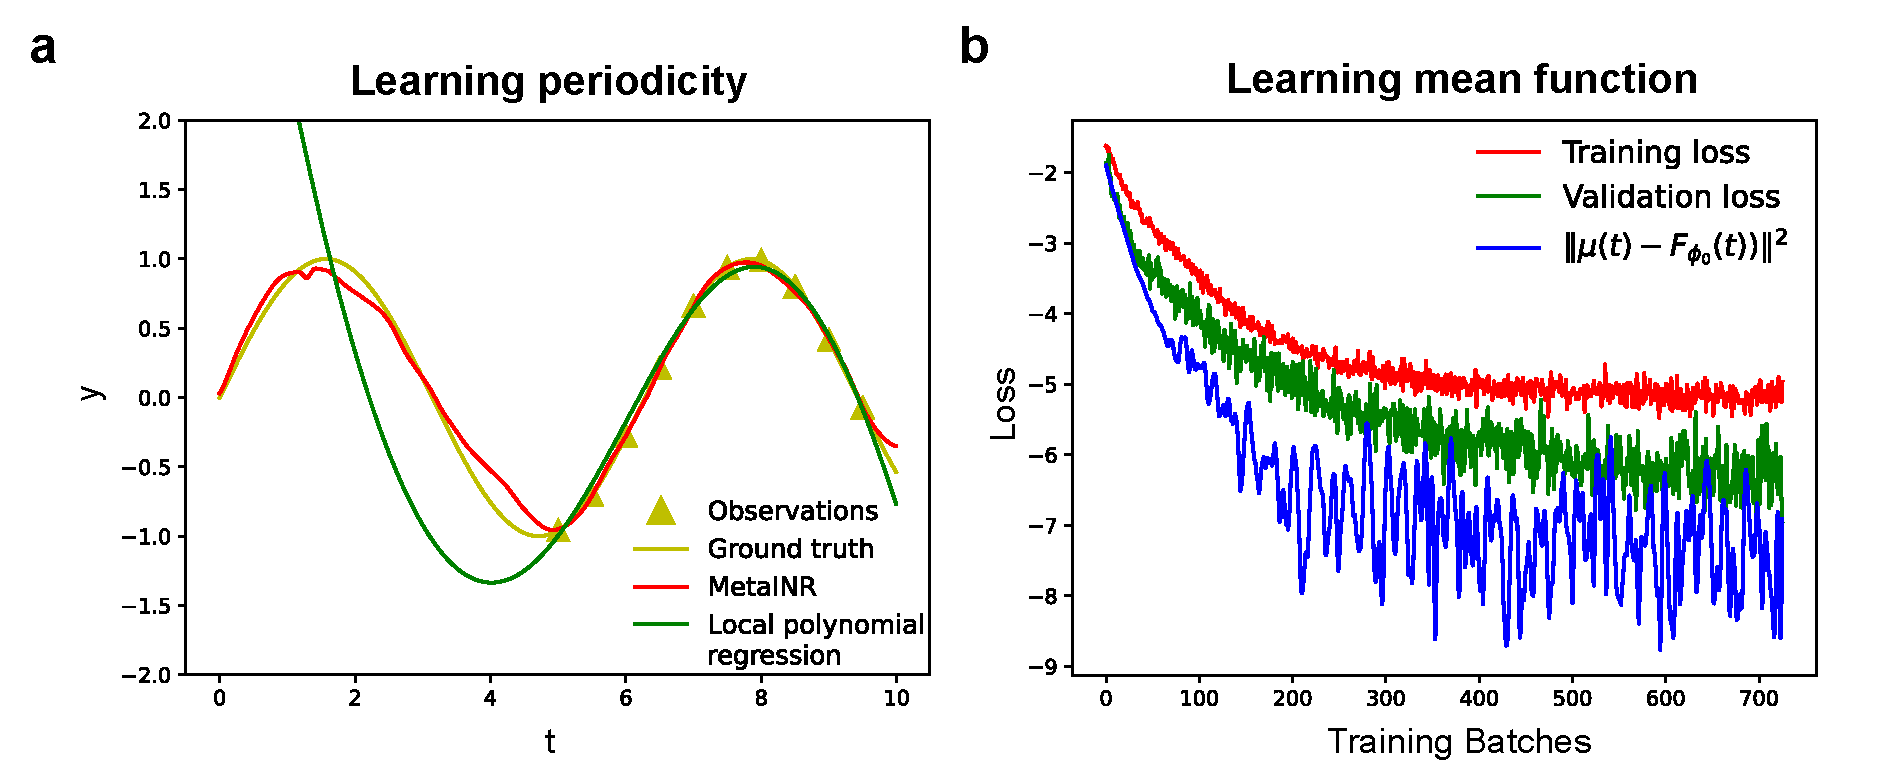
\includegraphics[width=\textwidth]{learning_commonalities.pdf}
  \caption{\textbf{Learning commonalities.} The figure illustrates two examples (periodicity \& mean function) of the ``shared characteristics'' that MAML learned among these tasks. 
  It is noticable that MetaINR is able to learn the periodicity between the interval $[0,5]$ while local polynomial regression totally misses this information. It is also clear that the meta-model gradually approximates the true mean function during the training process. }
  \label{Learning commonalities}
\end{figure}


% \begin{figure}
%   \centering
%   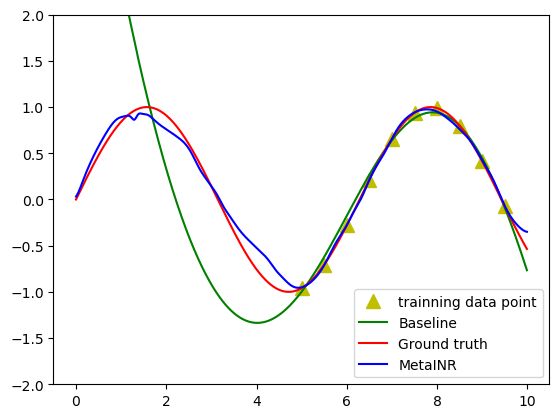
\includegraphics[width=0.5\textwidth]{learning_periodicity.png}
%   \caption{Learning periodicity}
% \end{figure}

% \begin{figure}
%   \centering
%   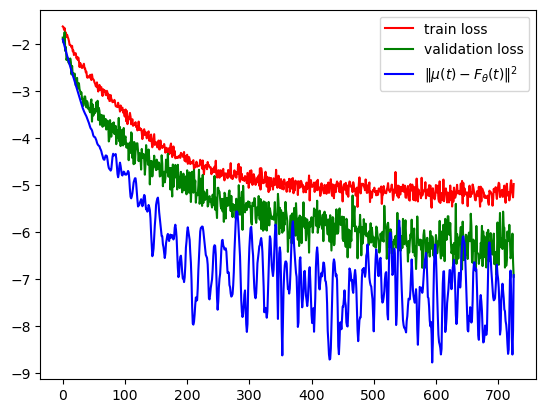
\includegraphics[width=0.5\textwidth]{learning_mean_loss.png}
%   \caption{Learning mean}
% \end{figure}



\textbf{Estimation of mean, covariance and principal components}
% 基于每个样本的MetaINR, 我们对这个人造数据集的均值函数,方差核和主成分进行了估计,结果如图3,4,5所示。
% 我们发现,以MetaINR为基础对三者的估计都远好于benchmarks。特别是在数据的边界处,即t接近0或10的位置,baseline的估计往往与真实值相差甚远,而基于MetaINR的估计却相对可靠。
Based on MetaINR workflow, we estimated the mean function, covariance kernel, and principal components of this synthetic dataset. 
As demonstrated in Figure \ref{Estimation for synthetic data},
the estimators based on MetaINR for all metrics significantly outperformed the benchmarks. 
%In sample recovery, Pre-smoothing method 在估计中没有考虑到其他样本带来的信息从而导致了在[0,1]区间中与真实值较大的偏离;PACE method 尽管在估计中考虑了所有样本的信息而产生相对较合理的样本恢复结果,但是恢复效果依然不如MetaINR,这可能和数据生成过程不满足PACE方法的假设条件有关。
%In mean function estimation, Pre-smoothing method 的估计等价于在不同的时间点给了所有样本相同的权重,但由于不同样本下观测点的数量和位置都不同,所以不同样本对给定时间点下的均值估计提供的信息是有差别的,因此基于Pre-smoothing method 的 均值估计依然存在较大偏差,而PACE和MetaINR的均值估计效果却相对较好。
%In covariance kernel estimation, Pre-smoothing 和 PACE 方法都与真实值产生了较大的差别。Particularly at the boundaries of the data, where $t$ approaches $0$ or $10$, the baseline estimators often deviated substantially from the true values, while the estimators based on MetaINR remained relatively reliable.在实际的实验过程中,我们发现这两个方法的估计结果对local polynomial regression 过程中 bandwidth的选取很敏感,因此,它们的估计是不够稳健的。
%In Principal component estimation, 我们发现这四种方法对于PC1都有着较好的估计,但Pre-smoothing 和 PACE 方法却都不能够较精准的捕捉PC2随时间的变动,而MetaINR 却近乎完美地估计了PC2。

In the context of sample recovery, 
the Pre-smoothing method did not take into account information from other samples in the estimation process, 
leading to significant deviations from the true values within the $[0,1]$ interval. 
On the other hand, although the PACE method considered information from all samples and produced relatively reasonable sample recovery results, 
its performance still falls short compared to MetaINR. 
This discrepancy may be attributed to the data generation process not meeting the assumptions of the PACE method.

Regarding mean function estimation, the Pre-smoothing method's estimation  assigned equal weights to all samples at different time points. 
However, since the number and positions of observed points vary among different samples, the information provided by different samples for estimating the mean at a given time point varies. 
As a result, mean estimation based on the Pre-smoothing method still exhibits significant bias, whereas the estimations from PACE and MetaINR are comparatively better.

In covariance kernel estimation, both Pre-smoothing and PACE methods exhibit substantial differences from the ground truth. 
% Specifically, near the boundaries of the data where $t$ approaches 0 or 10, 
% the baseline estimators often deviate significantly from the true values,
whereas the estimators based on MetaINR remain relatively reliable.
During our experiments, we observed that the estimation results of these two methods are highly sensitive to the selection of bandwidth in the local polynomial regression process, 
indicating that their estimations are not sufficiently robust.

Regarding Principal Component (PC) estimation, we found that all three methods performed well in estimating PC1. 
However, both the Pre-smoothing and PACE methods struggled to accurately capture the variation of PC2 over time, while MetaINR nearly perfectly estimated PC2.

\begin{figure}[htb]
  \centering
  \includegraphics[width=\textwidth]{synthetic_results.pdf}
  \caption{\textbf{Estimation for synthetic data.} The figure shows the results of the sample recovery and the estimation of mean function, covariance kernel and principal components in synthetic data. 
  In each plot, the horizontal axis represents time, and the vertical axis represents the corresponding variable's value. 
  It is clear that for all estimatiors, the performance of MetaINR is significantly better than that of Pre-smoothing and PACE methods. }
  \label{Estimation for synthetic data}
\end{figure}



% \begin{figure}
%   \centering
%   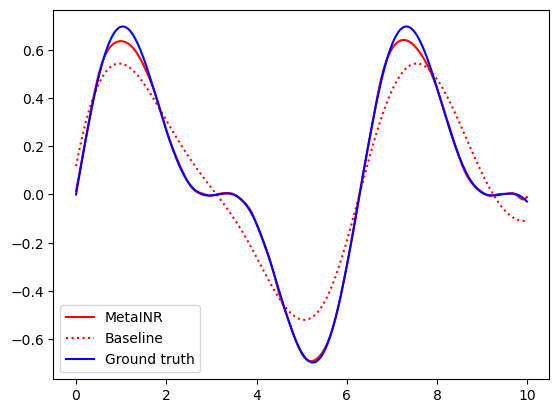
\includegraphics[width=0.5\textwidth]{mean.png}
%   \caption{Mean estimation}
% \end{figure}

% \begin{figure}
%   \centering
%   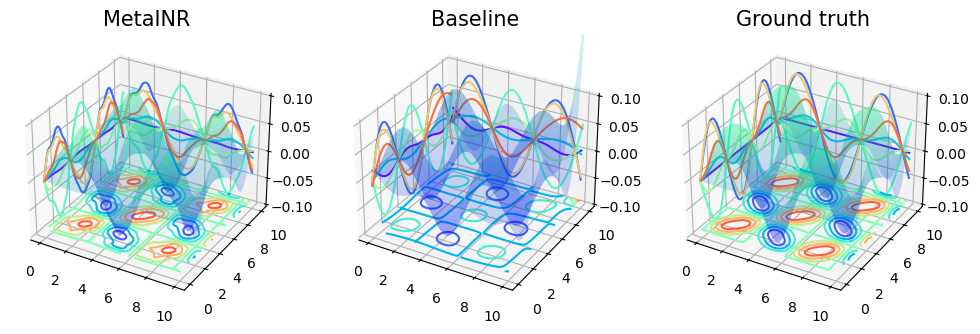
\includegraphics[width=\textwidth]{covariance.png}
%   \caption{Covariance estimation}
% \end{figure}

% \begin{figure}
%   \centering
%   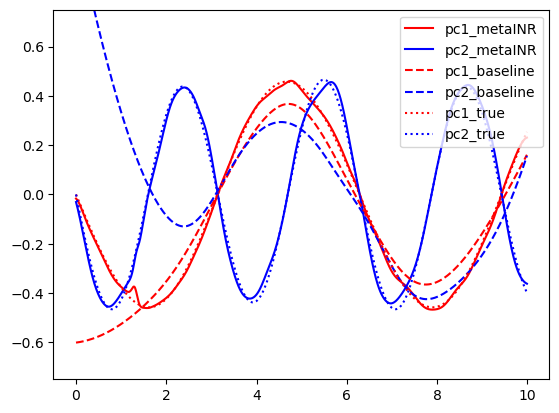
\includegraphics[width=0.5\textwidth]{fPCA.png}
%   \caption{FPCA}
% \end{figure}

%有待考虑
% \subsubsection{Metalearning+PACE Representation(dimensional reduction)}
% \subsubsection{Registration}

\subsection{Real-world data}
%CD4 count 的数据最好用
\textbf{Data description} 
In real-world scenarios, we apply MetaINR to the longitudinal data on primary biliary cirrhosis (PBC).
The data resulted from a Mayo Clinic trial that was conducted in 1974 to 1984, 
which is also described in \cite{markus1989efficacy}, \cite{fleming2013counting} and \cite{murtaugh1994primary}. 
They are available at \url{http://lib.stat.cmu.edu/datasets/pbc} and at a R package called ``survival''.
The data contain various sparsely and irregularly sampled covariates for each of 312 patients. 
Among these medical measurements,
serum bilirubin concentration is known to be elevated in the presence of chronic liver cirrhosis, such as PBC.
Therefore, it is important to analyze the time series data of bilirubin measurements for PBC prediction.
%所以预测并分析PBC数据的时间序列对病人十分重要
We extract data from the dataset for the initial 910 days, 
analyzing bilirubin measurements (in mg/dl) for different patients 
during the pre-onset phase. 
Our goal is to characterize the pattern of this measurement over time through estimates of mean function, covariance kernel and principal components.
In practice, we applied a logarithmic transformation to the bilirubin measurements and removed data for patients with a survival time less than 910 days.
% 因此,我们从数据集中截取了前910天的数据,对这发病前期不同病人的bilirubin measurements (in mg/dl)进行分析,期望通过主成分和均值的估计来刻画这个指标随时间变化的规律。
% 在实际操作中我们对bilirubin measurements取了对数变换,并且删除了存活时间小于910天的病人的数据。
A total of 260 patients in the study satisfied these criteria and only 2.9 observations per sample on average. 

\textbf{Parameters setting} 
In the PBC dataset, we set the initial parameters of SIREN $\omega_0=0.00005$, since the frequency spectrum data distribuiton is relatively low.
During the meta-learning training process, we equally divide the observations of each samples into support set and query set.
In the outer loop of MAML, we set the learning rate of the meta-model to 0.00005. 
In the inner loop of MAML, we set the model's learning rate to 0.00005 and the number of iterations for parameter optimization $Q=3$.
During subsequent gradient decent algorithm for sample recovery, the model's learning rate is set to 0.00005 and the total iterations is set to 500.

\textbf{Estimation of mean, covariance and principal components}
% 如图3展示了MetaINR在实际sparse functional dataset中的估计结果。我们发现虽然每个样本只有极少数的观测点,但是MetaINR却能较好地恢复样本。在统计量的估计方面,在这个特定的实际数据集中,metaINR有着与Baseline类似的估计效果。我们可以通过估计结果得到如下结论:在前910天的观测中,病人的serum bilirubin concentration先小幅下降,在400天左右,它又急剧上升(mean function)。不同病人之间serum bilirubin concentration除了在基础值上有差异外(pc1),从400天左右, 病人的serum bilirubin concentration之间出现较大的分化差异(pc2)。
Figure \ref{Estimation for real-world data} illustrates the estimation results of MetaINR on the real-world medical sparse functional dataset mentioned above. 
We observed that despite the minimal number of observations per sample, 
MetaINR can effectively recover the sample function. 
Regarding the estimation of statistical quantities, 
MetaINR demonstrates similar performance to the benchmarks in this specific real dataset.
\begin{figure}[htb]
  \centering
  \includegraphics[width=\textwidth]{real_results.pdf}
  \caption{\textbf{Estimation for real-world data.}The figure demonstates the results of the sample recovery (three typical examples), and the estimation of statistical quantities
  (mean function, covariance kernel and principal components) in real-world PBC data. 
  In each plot, the horizontal axis represents the observation time (days), and the vertical axis represents the value of logarithmic serum bilirubin concentration (mg/dl). 
  The estimated results are similar in all three methods.
  }
  \label{Estimation for real-world data}
\end{figure}

\textbf{Conclusion}
From the estimation results, we draw the following conclusions: 
Over the initial 910 days of observation, patients' serum bilirubin concentration initially experiences a slight decrease, 
followed by a sharp increase at around 400 days (mean function). 
Apart from differences in ``baseline values'' which remain invariant with time (PC1), 
significant divergence in serum bilirubin concentration among patients emerges around 400 days (PC2).


\section{Conclusion and future work}
% 我们展示了一个利用meta-learning的技术来处理sparse time series data的一个方法。通过meta-learning利用整个数据集的信息可以对只存在极少数观测点的样本进行MetaINR。基于MetaINR让一些原本只在稠密数据集中使用的functional data analysis的方法在sparse 数据集中变得可行。基于MetaINR的估计也为我们进一步分析sparse time series data提供了强大的工具。
In this paper, we have shown a method named MetaINR utilizing meta-learning to analyze sparse time series data. 
MetaINR enables the estimation of functional form samples with very few observation points by leveraging information from the entire dataset through meta-learning. 
The application of MetaINR makes functional data analysis (FDA) methods, which are typically used in dense datasets, feasible for sparse datasets. 
Therefore, MetaINR provides a novel tool for further analyzing sparse time series data.
% 在未来的研究中,我们希望可以利用MetaINR对其他原本只适用于稠密数据集的funcational data analysis的方法进行拓展,如FPLS,functional regression等。从而结合MetaINR和FDA的方法来建立针对sparse data的分析工具库。

In future research, we aim to extend the application of MetaINR to other functional data analysis methods that were initially designed for dense datasets, such as Functional Partial Least Squares Regression (FPLS), functional regression, registration and more.
We can also explore other algorithms of meta-learning, such as MANN \cite{santoro2016meta} and SNAIL \cite{mishra2017simple}, and compare the performances between them.
% This approach aims to build an analytical toolkit for sparse data by combining MetaINR with various functional data analysis methods.
\section{Appendix}

\subsection{Traditional FDA method for sparse functional data: PACE \cite{yao2005functional}} 
In functional data analysis, it is inappropriate to apply dense-data-based approaches directly on sparse dataset.
However, PACE method gives a alternative solution.

Although local polynomial regression is not suitable for a single sample with sparse observations, 
it is proved that one can employ this method to estimate the mean function and covariance operator consistently.
Specifically, given our sparse observations of dataset $D=\{(t_{ij},y_{ij})_{j=1}^{J_i}\}_{i=1}^n
$,
we can define the loss function to estimate mean function $\mu(t)$
$$
L_t^\mu(\beta)=\sum_{i=1}^n\sum_{j=1}^{J_i}\left[y_{ij}-\sum_{r=0}^R \beta_r\left(t-t_{ij}\right)^r\right]^2 K\left(\frac{t-t_{ij}}{h}\right),
$$
where $K(\cdot)$ is the kernel function and $h$ is the bandwidth which shoud be carefully chosen based on data.
By minimizing this function, we can get
$\beta_t=(\beta_0(t), \cdots, \beta_R(t))=arg\,min L_t^\mu(\beta)$. The estimator of mean function cam be defined as $\hat{\mu}(t)=\beta_0(t)$.
Similarly, to estimate the covariance kernel $c(t,s)$, we define the loss function 
$$
L^c_{t,s}(\beta)=\sum_{i=1}^n \sum_{1\leq j, l, \leq J_i} K_{t,s}(\frac{t-t_{ij}}{h}, \frac{s-t_{il}}{h}) \left[ g(t_{ij},t_{il})-f\left(\beta,(t,s),(t_{ij},t_{il})\right) \right]^2
$$
where
$$
g(t_{ij},t_{il})=(y_{ij}-\hat{\mu}(t_{ij}))(y_{il}-\hat{\mu}(t_{il}))
$$
$$
f\left(\beta,(t,s),(t_{ij},t_{il})\right)=\beta_0 + \beta_{11}(t-t_{ij})+\beta_{12}(s-t_{il})
$$
By minimization of $L_{t,s}^c(\beta)$, we obtain $(\beta_0(t),\beta_{11}(t),\beta_{12}(t))=arg\,min L_{t,s}^c(\beta)$. Then the estimator of the covariance kernel is defined as $\hat{c}(t,s)=\beta_0(t,s)$.
Under suitable conditions, including the fact that observations are random and well-spread, the estimators of mean function and covariance kernel are consistent \cite{yao2005functional} .
$$
\sup _{t \in \mathcal{T}}|\hat{\mu}(t)-\mu(t)|=O_p\left(\frac{1}{\sqrt{n} h_\mu}\right)
$$
$$
\sup _{t, s \in \mathcal{T}}|\hat{c}(s, t)-c(s, t)|=O_p\left(\frac{1}{\sqrt{n} h_G^2}\right)
$$
where $h_\mu$ and $h_G$ are bandwidths for estimating $\hat \mu$ and $\hat c$ satisfying
$$
\begin{aligned}
& h_\mu \rightarrow 0, n h_\mu^4 \rightarrow \infty, \text { and } n h_\mu^6<\infty; \\
& h_G \rightarrow 0, n h_G^6 \rightarrow \infty, \text { and } n h_G^8<\infty.
\end{aligned}
$$
Base on the estimated covariance kernel, we can derive the estimated  eigenvalues $\hat \lambda$ and eigenfunctions $\hat{\phi}_k(t)$ which are also consistent, \textit{i.e.}
$$
\left|\hat{\lambda}_k-\lambda_k\right|=O_p\left(\frac{1}{\sqrt{n} h_G^2}\right);
$$
$$
\sup _{t \in \mathcal{T}}\left|\hat{\phi}_k(t)-\phi_k(t)\right|=O_p\left(\frac{1}{\sqrt{n} h_G^2}\right), \quad k \in \mathcal{I}^{\prime}.
$$

Let 
$$\tilde{x}_i=\left(x_i\left(t_{i, 1}\right), \ldots, x_i\left(t_{i, J_i}\right)\right)^T, $$
$$\tilde{\mu}_i=\left(\widehat{\mu}\left(t_{i, 1}\right), \ldots, \widehat{\mu}\left(t_{i, J_i}\right)\right)^T, $$ 
$$\tilde{\phi}_{i, k}=\left(\widehat{\phi}_k\left(t_{i, 1}\right), \ldots, \widehat{\phi}_k\left(t_{i, J_i}\right)\right)^T.$$
Assume that $X_i(t)=\mu(t)+\sum_{k=1}^{\infty} a_{i k} \phi_k(t)$, with the $a_{i k} \sim N\left(0, \lambda_k\right)$,
Principal Analysis by Conditional Expectation (PACE) reconstructs each sample and estimates their scores by $\widehat{a}_{i k}=\hat{\mathbb{E}}\left(a_{i k} \mid \tilde{x}_i\right)$.
It can be shown that 
$$
\widehat{a}_{i, k}=\widehat{\lambda}_k \tilde{\phi}_{i, k}^T \Sigma_{x_i}^{-1}\left(\tilde{x}_i-\tilde{\mu}_i\right)
$$
where $\left\{\Sigma_{x_i}\right\}_{j, l}=\widehat{c}\left(t_{ij}, t_{il}\right)$.
The recovered sample can be represented by the first $K$ components 
$$\widehat{X}_i^K(t)=\widehat{\mu}(t)+\sum_{k=1}^K \widehat{a}_{i, k} \widehat{\phi}_k(t)$$
It can also be proved \cite{yao2005functional}  that under suitable conditions
$$
\lim _{n \rightarrow \infty} \hat{a}_{i k}={a}_{i k} \text { in probability, }
$$
and for all $t \in \mathcal{T}$,
$$
\lim _{K \rightarrow \infty} \lim _{n \rightarrow \infty} \widehat{X}_i^K(t)={X}_i(t) \text { in probability. }
$$


\subsection{The initialization scheme of SIREN \cite{sitzmann2020implicit}}

As discussed in the main text, SIREN is a restructured network architecture based on the traditional MLP, 
where the sine function replaces the original ReLU function as the activation function of the neural network. 
It can be represented as follows:
$$
\Phi(\mathbf{x})=\mathbf{W}_n\left(\phi_{n-1} \circ \phi_{n-2} \circ \ldots \circ \phi_0\right)(\mathbf{x})+\mathbf{b}_n, \quad \mathbf{x}_i \mapsto \phi_i\left(\mathbf{x}_i\right)=\sin \left(\mathbf{W}_i \mathbf{x}_i+\mathbf{b}_i\right)
$$
In practice, we need to carefully design its initialization scheme to ensure an effective training process. 
If we randomly initialize weights for SIREN, it can lead to inaccurate learning results and slow convergence speed.

The key principle of SIREN's initialization is to ensure that the output distribution of SIREN remains invariant regardless of the number of layers.
Consider the input of layer $\mathbf{x} \in \mathbb{R}^n$, which follows arcsine distribution
$$\mathbf{x}  \sim \operatorname{Arcsin}(-1,1)$$
$$(
X \sim \operatorname{Arcsin}(a, b), \text { with CDF: } F_X(x)=\frac{2}{\pi} \arcsin \left(\sqrt{\frac{x-a}{b-a}}\right) \text {, with } b>a
)$$
when we draw weights $\mathbf{W}$ whose components follow 
$$
w_i \sim Uniform (-\sqrt{6/n}, \sqrt{6/n}),
$$
it is proved that the dot product of weights and input of each layer converges to the normal distribution 
$$
\mathbf{w}^T \mathbf{x} \sim \mathcal{N}\left(0, 1\right),
$$
and the output of each layer (input of next layer) $\mathbf{x}^+=\phi_i\left(\mathbf{x}\right)=\sin \left(\mathbf{W} \mathbf{x}+\mathbf{b}\right)$ converges to an another arcsine distribution
$$\mathbf{x}^+  \sim \operatorname{Arcsin}(-1,1).$$
This property makes it posible that the output distribution of SIREN become invariant to the network's depth if we choose $\mathbf{W} \sim Uniform (-\sqrt{6/n}, \sqrt{6/n}).$


Besides, we also need to carefully choose the weights in the frist layer to match the frequency spectrum of the signal.
If the weights of first layer are too small, the activation sine function will degenerate to a linear function; if the weight are too large, the nonlinearity of activation function are too large:  Both of these extremes can lead to a decrease in SIREN's learning ability.
Therefore, we introduce a new factor $\omega_0$  and  draw the weights of first layer by
$$
\mathbf{W_0} = \omega_0 \times \mathbf{W},
$$
which should satisfy that the activation function of first layer $\sin \left(\omega_0 \cdot \mathbf{W} \mathbf{x_0}+\mathbf{b_0}\right)$ spans multiple periods over $[-1,1]$.

In practice, it is also found that the training speed of SIREN can be accelerated by using $\omega_0$ in the activation function of \textit{all} layers.
Replacing $\mathbf{W} \sim Uniform (-\sqrt{6/n}, \sqrt{6/n})$ by
$
\widehat {\mathbf{W}} \sim Uniform\left(-\sqrt{\frac{c}{\omega_0^2 n}}, \sqrt{\frac{c}{\omega_0^2 n}}\right)
$ 
will not only keep the activations constant but also boosts the gradients.


% \subsection{Experiments on other synthetic data}


\section*{Data and code availability}
PBC data used in this paper is available at \url{http://lib.stat.cmu.edu/datasets/pbc} , and it also can be found in a R package called ``survival''.
All the experimental code in this paper is available at \url{https://github.com/cbfcbf/code\_metaINR}.

\section*{Acknowledgments}
We express our gratitude to Prof. Mihaela van der Schaar for her invaluable supervision. 
Additionally, we extend our thanks to the research group members of the van der Scaar lab, Dr. Kasia Kobalczyk and Dr. Krzysztof Kacprzyk, for their insightful discussions and constructive suggestions. 
The input from these individuals significantly enhanced the quality of this paper.
\bibliographystyle{IEEEtran}      %IEEEtran为给定模板格式定义文件名
\bibliography{ref}



% \section{Submission of papers to NeurIPS 2023}

% \begin{tabular}{c|ccc|ccc|ccc}
%   \toprule
%   & \multicolumn{3}{c}{Action Delay~$\tau=\bar{\Delta}$ s}      & \multicolumn{3}{c}{Action Delay~$\tau=2\bar{\Delta}$ s}      &  \multicolumn{3}{c}{Action Delay~$\tau=3\bar{\Delta}$ s}               \\
%           Dynamics Model                  & Cartpole & Pendulum & Acrobot                   & Cartpole & Pendulum & Acrobot                     & Cartpole & Pendulum & Acrobot \\        
%   \midrule
%   Random & 0.0$\pm$0.0 & 0.0$\pm$8.39 & 0.0$\pm$9.06 & 0.0$\pm$0.0 & 0.0$\pm$0.0 & 0.0$\pm$8.11 & 0.0$\pm$0.0 & 0.0$\pm$8.91 & 0.0$\pm$0.0 \\
%   \midrule
%   Oracle & 100.0$\pm$0.03 & 100.0$\pm$2.94 & 100.0$\pm$1.8 & 100.0$\pm$0.04 & 100.0$\pm$2.6 & 100.0$\pm$2.19 & 100.0$\pm$0.11 & 100.0$\pm$1.52 & 100.0$\pm$2.45 \\
%   \bottomrule
% \end{tabular}

% Please read the instructions below carefully and follow them faithfully. \textbf{Important:} This year the checklist will be submitted separately from the main paper in OpenReview, please review it well ahead of the submission deadline: \url{https://neurips.cc/public/guides/PaperChecklist}.


% \subsection{Style}


% Papers to be submitted to NeurIPS 2023 must be prepared according to the
% instructions presented here. Papers may only be up to {\bf nine} pages long,
% including figures. Additional pages \emph{containing only acknowledgments and
% references} are allowed. Papers that exceed the page limit will not be
% reviewed, or in any other way considered for presentation at the conference.


% The margins in 2023 are the same as those in previous years.


% Authors are required to use the NeurIPS \LaTeX{} style files obtainable at the
% NeurIPS website as indicated below. Please make sure you use the current files
% and not previous versions. Tweaking the style files may be grounds for
% rejection.


% \subsection{Retrieval of style files}


% The style files for NeurIPS and other conference information are available on
% the website at
% \begin{center}
%   \url{http://www.neurips.cc/}
% \end{center}
% The file \verb+neurips_2023.pdf+ contains these instructions and illustrates the
% various formatting requirements your NeurIPS paper must satisfy.


% The only supported style file for NeurIPS 2023 is \verb+neurips_2023.sty+,
% rewritten for \LaTeXe{}.  \textbf{Previous style files for \LaTeX{} 2.09,
%   Microsoft Word, and RTF are no longer supported!}


% The \LaTeX{} style file contains three optional arguments: \verb+final+, which
% creates a camera-ready copy, \verb+preprint+, which creates a preprint for
% submission to, e.g., arXiv, and \verb+nonatbib+, which will not load the
% \verb+natbib+ package for you in case of package clash.


% \paragraph{Preprint option}
% If you wish to post a preprint of your work online, e.g., on arXiv, using the
% NeurIPS style, please use the \verb+preprint+ option. This will create a
% nonanonymized version of your work with the text ``Preprint. Work in progress.''
% in the footer. This version may be distributed as you see fit, as long as you do not say which conference it was submitted to. Please \textbf{do
%   not} use the \verb+final+ option, which should \textbf{only} be used for
% papers accepted to NeurIPS. 


% At submission time, please omit the \verb+final+ and \verb+preprint+
% options. This will anonymize your submission and add line numbers to aid
% review. Please do \emph{not} refer to these line numbers in your paper as they
% will be removed during generation of camera-ready copies.


% The file \verb+neurips_2023.tex+ may be used as a ``shell'' for writing your
% paper. All you have to do is replace the author, title, abstract, and text of
% the paper with your own.


% The formatting instructions contained in these style files are summarized in
% Sections \ref{gen_inst}, \ref{headings}, and \ref{others} below.


% \section{General formatting instructions}
% \label{gen_inst}


% The text must be confined within a rectangle 5.5~inches (33~picas) wide and
% 9~inches (54~picas) long. The left margin is 1.5~inch (9~picas).  Use 10~point
% type with a vertical spacing (leading) of 11~points.  Times New Roman is the
% preferred typeface throughout, and will be selected for you by default.
% Paragraphs are separated by \nicefrac{1}{2}~line space (5.5 points), with no
% indentation.


% The paper title should be 17~point, initial caps/lower case, bold, centered
% between two horizontal rules. The top rule should be 4~points thick and the
% bottom rule should be 1~point thick. Allow \nicefrac{1}{4}~inch space above and
% below the title to rules. All pages should start at 1~inch (6~picas) from the
% top of the page.


% For the final version, authors' names are set in boldface, and each name is
% centered above the corresponding address. The lead author's name is to be listed
% first (left-most), and the co-authors' names (if different address) are set to
% follow. If there is only one co-author, list both author and co-author side by
% side.


% Please pay special attention to the instructions in Section \ref{others}
% regarding figures, tables, acknowledgments, and references.


% \section{Headings: first level}
% \label{headings}


% All headings should be lower case (except for first word and proper nouns),
% flush left, and bold.


% First-level headings should be in 12-point type.


% \subsection{Headings: second level}


% Second-level headings should be in 10-point type.


% \subsubsection{Headings: third level}


% Third-level headings should be in 10-point type.


% \paragraph{Paragraphs}


% There is also a \verb+\paragraph+ command available, which sets the heading in
% bold, flush left, and inline with the text, with the heading followed by 1\,em
% of space.


% \section{Citations, figures, tables, references}
% \label{others}


% These instructions apply to everyone.


% \subsection{Citations within the text}


% The \verb+natbib+ package will be loaded for you by default.  Citations may be
% author/year or numeric, as long as you maintain internal consistency.  As to the
% format of the references themselves, any style is acceptable as long as it is
% used consistently.


% The documentation for \verb+natbib+ may be found at
% \begin{center}
%   \url{http://mirrors.ctan.org/macros/latex/contrib/natbib/natnotes.pdf}
% \end{center}
% Of note is the command \verb+\citet+, which produces citations appropriate for
% use in inline text.  For example,
% \begin{verbatim}
%    \citet{hasselmo} investigated\dots
% \end{verbatim}
% produces
% \begin{quote}
%   Hasselmo, et al.\ (1995) investigated\dots
% \end{quote}


% If you wish to load the \verb+natbib+ package with options, you may add the
% following before loading the \verb+neurips_2023+ package:
% \begin{verbatim}
%    \PassOptionsToPackage{options}{natbib}
% \end{verbatim}


% If \verb+natbib+ clashes with another package you load, you can add the optional
% argument \verb+nonatbib+ when loading the style file:
% \begin{verbatim}
%    \usepackage[nonatbib]{neurips_2023}
% \end{verbatim}


% As submission is double blind, refer to your own published work in the third
% person. That is, use ``In the previous work of Jones et al.\ [4],'' not ``In our
% previous work [4].'' If you cite your other papers that are not widely available
% (e.g., a journal paper under review), use anonymous author names in the
% citation, e.g., an author of the form ``A.\ Anonymous'' and include a copy of the anonymized paper in the supplementary material.


% \subsection{Footnotes}


% Footnotes should be used sparingly.  If you do require a footnote, indicate
% footnotes with a number\footnote{Sample of the first footnote.} in the
% text. Place the footnotes at the bottom of the page on which they appear.
% Precede the footnote with a horizontal rule of 2~inches (12~picas).


% Note that footnotes are properly typeset \emph{after} punctuation
% marks.\footnote{As in this example.}


% \subsection{Figures}


% \begin{figure}
%   \centering
%   \fbox{\rule[-.5cm]{0cm}{4cm} \rule[-.5cm]{4cm}{0cm}}
%   \caption{Sample figure caption.}
% \end{figure}


% All artwork must be neat, clean, and legible. Lines should be dark enough for
% purposes of reproduction. The figure number and caption always appear after the
% figure. Place one line space before the figure caption and one line space after
% the figure. The figure caption should be lower case (except for first word and
% proper nouns); figures are numbered consecutively.


% You may use color figures.  However, it is best for the figure captions and the
% paper body to be legible if the paper is printed in either black/white or in
% color.


% \subsection{Tables}


% All tables must be centered, neat, clean and legible.  The table number and
% title always appear before the table.  See Table~\ref{sample-table}.


% Place one line space before the table title, one line space after the
% table title, and one line space after the table. The table title must
% be lower case (except for first word and proper nouns); tables are
% numbered consecutively.


% Note that publication-quality tables \emph{do not contain vertical rules.} We
% strongly suggest the use of the \verb+booktabs+ package, which allows for
% typesetting high-quality, professional tables:
% \begin{center}
%   \url{https://www.ctan.org/pkg/booktabs}
% \end{center}
% This package was used to typeset Table~\ref{sample-table}.


% \begin{table}
%   \caption{Sample table title}
%   \label{sample-table}
%   \centering
%   \begin{tabular}{lll}
%     \toprule
%     \multicolumn{2}{c}{Part}                   \\
%     \cmidrule(r){1-2}
%     Name     & Description     & Size ($\mu$m) \\
%     \midrule
%     Dendrite & Input terminal  & $\sim$100     \\
%     Axon     & Output terminal & $\sim$10      \\
%     Soma     & Cell body       & up to $10^6$  \\
%     \bottomrule
%   \end{tabular}
% \end{table}

% \subsection{Math}
% Note that display math in bare TeX commands will not create correct line numbers for submission. Please use LaTeX (or AMSTeX) commands for unnumbered display math. (You really shouldn't be using \$\$ anyway; see \url{https://tex.stackexchange.com/questions/503/why-is-preferable-to} and \url{https://tex.stackexchange.com/questions/40492/what-are-the-differences-between-align-equation-and-displaymath} for more information.)

% \subsection{Final instructions}

% Do not change any aspects of the formatting parameters in the style files.  In
% particular, do not modify the width or length of the rectangle the text should
% fit into, and do not change font sizes (except perhaps in the
% \textbf{References} section; see below). Please note that pages should be
% numbered.


% \section{Preparing PDF files}


% Please prepare submission files with paper size ``US Letter,'' and not, for
% example, ``A4.''


% Fonts were the main cause of problems in the past years. Your PDF file must only
% contain Type 1 or Embedded TrueType fonts. Here are a few instructions to
% achieve this.


% \begin{itemize}


% \item You should directly generate PDF files using \verb+pdflatex+.


% \item You can check which fonts a PDF files uses.  In Acrobat Reader, select the
%   menu Files$>$Document Properties$>$Fonts and select Show All Fonts. You can
%   also use the program \verb+pdffonts+ which comes with \verb+xpdf+ and is
%   available out-of-the-box on most Linux machines.


% \item \verb+xfig+ "patterned" shapes are implemented with bitmap fonts.  Use
%   "solid" shapes instead.


% \item The \verb+\bbold+ package almost always uses bitmap fonts.  You should use
%   the equivalent AMS Fonts:
% \begin{verbatim}
%    \usepackage{amsfonts}
% \end{verbatim}
% followed by, e.g., \verb+\mathbb{R}+, \verb+\mathbb{N}+, or \verb+\mathbb{C}+
% for $\mathbb{R}$, $\mathbb{N}$ or $\mathbb{C}$.  You can also use the following
% workaround for reals, natural and complex:
% \begin{verbatim}
%    \newcommand{\RR}{I\!\!R} %real numbers
%    \newcommand{\Nat}{I\!\!N} %natural numbers
%    \newcommand{\CC}{I\!\!\!\!C} %complex numbers
% \end{verbatim}
% Note that \verb+amsfonts+ is automatically loaded by the \verb+amssymb+ package.


% \end{itemize}


% If your file contains type 3 fonts or non embedded TrueType fonts, we will ask
% you to fix it.


% \subsection{Margins in \LaTeX{}}


% Most of the margin problems come from figures positioned by hand using
% \verb+\special+ or other commands. We suggest using the command
% \verb+\includegraphics+ from the \verb+graphicx+ package. Always specify the
% figure width as a multiple of the line width as in the example below:
% \begin{verbatim}
%    \usepackage[pdftex]{graphicx} ...
%    \includegraphics[width=0.8\linewidth]{myfile.pdf}
% \end{verbatim}
% See Section 4.4 in the graphics bundle documentation
% (\url{http://mirrors.ctan.org/macros/latex/required/graphics/grfguide.pdf})


% A number of width problems arise when \LaTeX{} cannot properly hyphenate a
% line. Please give LaTeX hyphenation hints using the \verb+\-+ command when
% necessary.


% \begin{ack}
% Use unnumbered first level headings for the acknowledgments. All acknowledgments
% go at the end of the paper before the list of references. Moreover, you are required to declare
% funding (financial activities supporting the submitted work) and competing interests (related financial activities outside the submitted work).
% More information about this disclosure can be found at: \url{https://neurips.cc/Conferences/2023/PaperInformation/FundingDisclosure}.


% Do {\bf not} include this section in the anonymized submission, only in the final paper. You can use the \texttt{ack} environment provided in the style file to autmoatically hide this section in the anonymized submission.
% \end{ack}



% \section{Supplementary Material}

% Authors may wish to optionally include extra information (complete proofs, additional experiments and plots) in the appendix. All such materials should be part of the supplemental material (submitted separately) and should NOT be included in the main submission.


% \section*{References}


% References follow the acknowledgments in the camera-ready paper. Use unnumbered first-level heading for
% the references. Any choice of citation style is acceptable as long as you are
% consistent. It is permissible to reduce the font size to \verb+small+ (9 point)
% when listing the references.
% Note that the Reference section does not count towards the page limit.
% \medskip


% {
% \small


% [1] Alexander, J.A.\ \& Mozer, M.C.\ (1995) Template-based algorithms for
% connectionist rule extraction. In G.\ Tesauro, D.S.\ Touretzky and T.K.\ Leen
% (eds.), {\it Advances in Neural Information Processing Systems 7},
% pp.\ 609--616. Cambridge, MA: MIT Press.


% [2] Bower, J.M.\ \& Beeman, D.\ (1995) {\it The Book of GENESIS: Exploring
%   Realistic Neural Models with the GEneral NEural SImulation System.}  New York:
% TELOS/Springer--Verlag.


% [3] Hasselmo, M.E., Schnell, E.\ \& Barkai, E.\ (1995) Dynamics of learning and
% recall at excitatory recurrent synapses and cholinergic modulation in rat
% hippocampal region CA3. {\it Journal of Neuroscience} {\bf 15}(7):5249-5262.
% }

% %%%%%%%%%%%%%%%%%%%%%%%%%%%%%%%%%%%%%%%%%%%%%%%%%%%%%%%%%%%%


 \end{document}